\documentclass[sn-mathphys-num]{sn-jnl}
%% Builds offline with the bundled sn-jnl.cls SHIM. For Springer submission,
%% delete sn-jnl.cls and use the OFFICIAL class -- this file needs no changes.

\usepackage{siunitx}
\usepackage{placeins}
\usepackage[colorlinks=true,linkcolor=black,citecolor=black,urlcolor=blue!55!black]{hyperref}
\usepackage[capitalise,noabbrev]{cleveref}
\usetikzlibrary{arrows.meta,positioning,calc,fit,backgrounds}

\sisetup{detect-all,group-minimum-digits=4}

\definecolor{proxyred}{HTML}{E4572E}
\definecolor{compblue}{HTML}{2E86AB}
\definecolor{aftergreen}{HTML}{2E9E5B}
\definecolor{panel}{HTML}{F4F6F8}

\newcommand{\PCLN}{\textsc{Pcln}}
\newcommand{\PLS}{\mathrm{PLS}}
\newcommand{\DP}{\mathrm{DP}}
\newcommand{\A}{A}
\newcommand{\Exp}{\mathbb{E}}
\newcommand{\Real}{\mathbb{R}}
\newcommand{\given}{\,\vert\,}
\newcommand{\Nec}{\mathrm{Nec}}
\newcommand{\Suf}{\mathrm{Suf}}
\newcommand{\Cau}{\mathrm{Cau}}
\newcommand{\xcf}{x^{\mathrm{CF}}}
\newcommand{\xsuf}{x^{\mathrm{SUF}}}
\newcommand{\cmark}{{\color{aftergreen}\checkmark}}
\newcommand{\xmark}{{\color{proxyred}\(\boldsymbol\times\)}}
\newcommand{\pmark}{{\color{black!55}$\sim$}}

\title{Causal Certificates for Proxy Discrimination: An Exact Bridge from Demographic Parity to Per-Decision Necessity and Sufficiency}

\author*[1]{\fnm{Le Vo Minh} \sur{Thu}}\email{lvmthu@hcmus.edu.vn}
\author[1]{\fnm{Le Hoai} \sur{Bac}}
\author[1]{\fnm{Tran Thai} \sur{Son}}
\affil[1]{\orgdiv{Faculty of Information Technology}, \orgname{University of Science, Vietnam National University Ho Chi Minh City (HCMUS, VNU-HCM)}, \orgaddress{\city{Ho Chi Minh City}, \country{Vietnam}}}

\abstract{A fairness audit lives in two worlds that rarely meet. Group-fairness
metrics such as demographic parity and equal opportunity are population averages,
so they can say that a process is biased but cannot explain or justify any single
decision. Per-instance explanations such as Shapley values and counterfactuals
describe one decision, yet they carry no fairness guarantee and do not aggregate
to any group quantity. Proxy discrimination, in which a model re-learns a
withheld protected attribute $A$ through correlated features
($A\!\to\!X\!\to\!\hat Y$), is exactly the phenomenon that needs both worlds at
once, because it calls for a per-applicant answer to the question of whether
someone was rejected because of a proxy, and that answer must be tied to the
population disparity. We provide that bridge. Starting from the single
local-accuracy property of additive explanations, we derive an exact per-feature
decomposition of the demographic-parity gap, a localizer that recovers the proxy
channel, and per-decision causal certificates that state the necessity,
sufficiency, and causation of the proxy channel for an individual outcome through
a directed, label-free counterfactual. Our central result is a consistency
theorem showing that the individual causal effect averages back exactly to the
per-cluster term of the group decomposition, so that the per-decision explanation
and the population metric become two views of one quantity. We further show that
the attribution must be interventional, because a conditional (observational)
Shapley estimator spreads proxy credit onto correlated legitimate features and
biases the split between direct and indirect effects, whereas the interventional
estimator stays faithful while preserving the exact decomposition. On a
controlled recruitment testbed with ground-truth proxies, localization is exact
(average precision $1.00$), the certificate finds that $15.7\%$ of disadvantaged
rejections are caused by the proxy channel, and the certificate stays
conservative precisely when the channel also carries legitimate signal. The same
decomposition powers a targeted repair that cuts the parity gap by $92\%$ at no
more than $0.02$ AUC cost, and we report openly that minimizing parity can
enlarge the equal-opportunity gap. On the real, published FairCVdb benchmark the
audit transfers cleanly, localizing the demographic embedding with precision
$1.00$ and cutting the measured parity gap by $60\%$ at an AUC cost of $0.014$.}

\keywords{algorithmic fairness, proxy discrimination, actual causation, necessity and sufficiency, Shapley values, causal mediation}

\begin{document}
\maketitle

\section{Introduction}
\label{sec:intro}

Consider an automated hiring screen that, by policy, is never shown the
applicant's gender. A regulator asks two questions. The first is about the
\emph{system}: ``does this screen disadvantage women?'' The second is about a
\emph{person}: ``was \emph{this} applicant rejected because of her gender?'' Today
these questions are answered by different, disconnected tools. Group-fairness
metrics answer the first with a single number, a demographic-parity or
equal-opportunity gap, but that number is a population average and says nothing
about any individual file. Per-instance explainability answers the second with a
Shapley attribution or a counterfactual, but those carry no fairness semantics
and do not add up to the group gap. Neither tool, alone, can certify that a
particular rejection was \emph{caused} by a protected attribute the model was
never given.

This disconnect is most acute for \emph{proxy discrimination}. Two influential
benchmarks make the mechanism vivid. \emph{FairCVtest}~\cite{pena2020faircv,
pena2023human} builds a multimodal recruitment testbed in which a blind,
competency-only score is corrupted by a group penalty, and shows that a model
denied the protected attribute reconstructs it from correlated channels.
\emph{FairJob}~\cite{vladimirova2024fairjob}, a million-row Criteo log, reports
the same on real data: an ``unaware'' model matches an ``unfair'' one because the
attribute is recovered from the feature vector. Both summarize the effect as a
causal chain $A\!\to\!X\!\to\!\hat Y$. Yet the diagnosis stops at the population:
neither says \emph{which} features carry the attribute, \emph{how much} each
contributes to the measured gap, and, most importantly, whether the chain is the
\emph{actual cause} of any individual's outcome.

The gap between these two views is not merely technical. Anti-discrimination law
distinguishes disparate \emph{impact}, a population-level disparity, from disparate
\emph{treatment}, the use of a protected attribute in an individual
decision~\cite{barocas2016disparate}, and a defensible audit must speak to both.
A regulator who learns only that a screen rejects women at a higher rate cannot
tell whether a given applicant has a grievance, and a developer who sees only a
Shapley attribution for one applicant cannot tell whether the pattern is systemic.
The two numbers can even point in opposite directions: a model may show a sizeable
group gap while no single decision turns on the proxy, or conversely concentrate
its harm in a few proxy-driven decisions that a population average dilutes to
near-invisibility. What is missing is an object that is simultaneously a statement
about a person and a statement about the population, with a guarantee that the two
agree.

\paragraph{This paper.}
We close the loop between the population and the person. Our key observation is
that one object, the additive (Shapley) decomposition of the model's score, can
be read at both scales as long as it is paired with the right counterfactual
operator. We use a directed, label-free intervention that removes the protected
direction inside a localized proxy channel, and we show that this single operator
yields a complete account of proxy discrimination, from the group gap down to the
individual decision.

Four questions guide the work, and each follows directly from a gap left open by
the diagnostic benchmarks~\cite{pena2020faircv,vladimirova2024fairjob} and the
broader fairness-explanation literature~\cite{mehrabi2021survey}. The first
concerns \emph{localization}: among the many explanation methods available, which
one most faithfully recovers the proxy channel that a model actually relies on,
rather than features that are merely predictive or merely correlated with the
protected attribute? The second concerns \emph{attribution}: once a channel is
found, how should per-feature credit be assigned so that the decomposition of the
group disparity stays causally faithful instead of being smeared across
correlated features? The third concerns \emph{per-decision causation}: can we
certify, for a single applicant, that the proxy channel was a genuine cause, both
necessary and sufficient, of their outcome, and can that certificate stay
cautious when the same channel also does legitimate work? The fourth concerns
\emph{consistency}: do the per-decision certificates add back up exactly to the
population fairness metric, so that the individual view and the group view can
never disagree? Our answers combine into a single recommended pipeline, namely
PLS localization, interventional Shapley attribution, and a directed-counterfactual
certificate, and we show that this combination outperforms the natural
single-method baselines.

\paragraph{Contributions.}
\begin{enumerate}[leftmargin=1.6em,itemsep=0.22em,topsep=0.25em]
  \item \textbf{An exact group decomposition (\cref{prop:decomp}).} By
        local accuracy alone, the demographic-parity gap of the score equals the
        sum of per-feature terms $\Delta_j=\Exp[\phi_j\given A{=}1]-\Exp[\phi_j\given A{=}0]$,
        with no residual, giving an auditable ledger for the $A\!\to\!X\!\to\!\hat Y$
        claim.
  \item \textbf{Per-decision causal certificates (\cref{def:cert}).} Through a
        directed counterfactual we define the \emph{necessity}, \emph{sufficiency},
        and \emph{causation} of the proxy channel for an individual decision,
        importing the necessity/sufficiency calculus of actual
        causation~\cite{halpern2005causes,watson2021local} into fairness auditing.
        A decision that is both necessary- and sufficient-attributable is
        \emph{caused} by the proxy channel.
  \item \textbf{A consistency theorem (\cref{thm:bridge}).} The individual causal
        effect averages back \emph{exactly} to the per-cluster term of the group
        decomposition. The per-decision certificate and the group metric are two
        projections of one quantity, which is the formal bridge between the regulator's
        two questions.
  \item \textbf{The certificate is honest under mixing.} When the proxy channel
        also carries legitimate signal, sufficiency drops and the causal rate
        falls \emph{below} necessity: the certificate refuses to over-attribute,
        exactly when it should.
  \item \textbf{Faithful attribution must be interventional.} Reading the gap as
        a natural indirect (proxy-path) plus direct effect, we show a conditional
        (observational) Shapley estimator smears proxy credit onto correlated
        legitimate features and so biases the split between direct and indirect effects, while the
        interventional estimator stays faithful, both preserving the exact
        decomposition.
  \item \textbf{A targeted repair and an honest tension.} The same localization
        drives a surgical neutralizer that cuts the parity gap by $92\%$ at
        $\le0.02$ AUC cost on a ground-truth testbed, with A-direction
        orthogonalization preserving utility that deletion destroys; we show, not
        hide, that the repair can worsen equal opportunity.
\end{enumerate}

\noindent
We validate every claim with injected ground truth on a faithful FairCVtest-recipe
testbed, confirm the audit on the real, published FairCVdb, and ship runnable
transfer scripts plus an interactive auditor.

\section{Related Work}
\label{sec:related}

\paragraph{Group fairness and unawareness.}
That deleting $A$ does not remove its influence is foundational~\cite{dwork2012fairness,
barocas2017fairness}: redundant encodings survive. Parity is enforced by
reductions~\cite{agarwal2018reductions}, post-processing~\cite{hardt2016equality},
or data repair~\cite{feldman2015certifying}; all act on the whole feature vector
and report population rates. We instead \emph{attribute} the gap and act on the
specific channel responsible.

\paragraph{Proxy and causal fairness.}
FairCVtest~\cite{pena2020faircv,pena2023human} and FairJob~\cite{vladimirova2024fairjob}
establish proxy leakage empirically; SensitiveNets~\cite{serna2021sensitivenets}
learns agnostic representations. Counterfactual
fairness~\cite{kusner2017counterfactual} and causal fairness
testing~\cite{galhotra2017fairness} reason about $A$'s effect but require a
structural causal model. Our certificates need only a trained scorer, an
explainer, and the protected attribute on an audit split, with no structural causal model, yet still
deliver necessity/sufficiency in the sense of actual
causation~\cite{pearl2009causality,halpern2005causes}.

\paragraph{Explanations, necessity, and sufficiency.}
SHAP~\cite{lundberg2017shap,strumbelj2014explaining} supplies additive
attributions whose local accuracy we exploit. Counterfactual
explanations~\cite{wachter2017counterfactual} edit features to flip a decision;
necessity/sufficiency have been proposed as the right axes for \emph{local}
explanation quality~\cite{watson2021local} and, for rationales, as
comprehensiveness and sufficiency~\cite{deyoung2020eraser}. We are, to our
knowledge, the first to (a) tie these per-decision causal axes specifically to a
\emph{localized proxy channel} and (b) prove they aggregate exactly to a
group-fairness metric. Calibration~\cite{guo2017calibration} completes our
evaluation triad.

\paragraph{Fairness criteria and their tensions.}
The fairness literature offers many criteria, and several are mutually
exclusive: a calibrated score generally cannot equalize both false-positive and
false-negative rates across groups when base rates
differ~\cite{kleinberg2017inherent,chouldechova2017fair}, and the broader space
of definitions has been catalogued and shown to encode incompatible normative
choices~\cite{verma2018fairness,corbett2018measure,mehrabi2021survey}. Our
contribution is orthogonal to the choice of criterion: the same score
decomposition can be conditioned to target demographic parity or, by restricting
to the qualified subpopulation, equal opportunity. We surface the
parity-versus-opportunity tension empirically rather than legislating it away.

\paragraph{Reliability of post hoc explanations.}
The explanation methods an auditor might reach for are not interchangeable.
Saliency maps can be insensitive to the model and the data they purport to
explain~\cite{adebayo2018sanity}; LIME and kernel SHAP can be adversarially
manipulated to hide bias~\cite{slack2020fooling}; and Shapley attributions differ
sharply depending on whether absent features are marginalized interventionally or
conditionally~\cite{sundararajan2020many,janzing2020feature,aas2021explaining},
a divergence we measure directly for proxy auditing. Quantitative input
influence~\cite{datta2016algorithmic} and tree-specific
attributions~\cite{lundberg2020local} share the same dependence on the reference
distribution. Our localizer is built to be robust to exactly the failure modes
these works document, and we benchmark it against the natural single-signal
alternatives.

\paragraph{Recourse and actionability.}
Counterfactual explanations are also the basis of algorithmic
recourse~\cite{karimi2022survey,wachter2017counterfactual}, which asks what an
individual could change to flip an unfavourable decision. Our directed
counterfactual is the dual object: rather than changing the applicant, it changes
the model's reliance on the proxy, and the same operator that issues the
per-decision certificate also defines the repair.

\Cref{tab:capabilities} positions our method against the most relevant
families. Diagnostic benchmarks establish that proxy leakage exists but localize
nothing; in-processing and post-processing methods repair fairness but act on the
whole feature vector and report only population rates; counterfactual fairness
reasons causally but needs a structural causal model (SCM) and yields no group
decomposition; metric-attribution methods decompose a fairness number but stop at
the population. ProxyAudit is the only entry that delivers all five capabilities
at once, namely localization, an exact group decomposition, a per-decision
necessity/sufficiency certificate, a population-to-individual consistency
guarantee, and a targeted repair, all without assuming a structural causal model.

\begin{table}[tbp]
\centering
\caption{Where ProxyAudit sits among fairness-analysis families. \cmark{}~=~yes,
\pmark{}~=~partial, \xmark{}~=~no.}
\label{tab:capabilities}
\small
\setlength{\tabcolsep}{4.5pt}
\begin{tabular}{lcccccc}
\toprule
\textbf{Method / family} & \shortstack{Per-feature\\localization} & \shortstack{Exact group\\decomposition} & \shortstack{Per-decision\\certificate} & \shortstack{Necessity \&\\sufficiency} & \shortstack{SCM-\\free} & \shortstack{Targeted\\repair}\\
\midrule
Diagnostic benchmarks \cite{pena2020faircv,vladimirova2024fairjob} & \xmark & \xmark & \xmark & \xmark & \cmark & \xmark\\
In-/post-processing \cite{agarwal2018reductions,hardt2016equality} & \xmark & \xmark & \xmark & \xmark & \cmark & \pmark\\
Counterfactual fairness \cite{kusner2017counterfactual} & \xmark & \xmark & \pmark & \pmark & \xmark & \xmark\\
Metric attribution \cite{begley2020explainability} & \pmark & \cmark & \xmark & \xmark & \cmark & \xmark\\
Local Nec./Suf.\ \cite{watson2021local} & \xmark & \xmark & \cmark & \cmark & \cmark & \xmark\\
\textbf{ProxyAudit (ours)} & \cmark & \cmark & \cmark & \cmark & \cmark & \cmark\\
\bottomrule
\end{tabular}
\end{table}

\section{From Group Disparity to Per-Decision Causation}
\label{sec:theory}

We develop the theory in one arc: an exact group decomposition
(\cref{sec:decomp}), the directed counterfactual that localizes and repairs the
channel (\cref{sec:operator}), the per-decision causal certificates built on that
counterfactual (\cref{sec:cert}), and the theorem that ties the two scales
together (\cref{sec:bridge}).

\subsection{Setup}
Let $f:\Real^d\!\to\!\Real$ be a trained scorer whose score (logit) we audit, and
$A\in\{0,1\}$ a protected attribute \emph{withheld} from $f$. Decisions select the
top-$\tau$ fraction by score, which is the natural operating point when a fixed number of
positions is filled, and we use one budget $\tau$ for every comparison so that
disparities are measured at equal selection rates. An additive explainer gives
$\phi_j(x)$, the contribution of feature $j$ to $f(x)$, with base value $\phi_0$
and local accuracy $f(x)=\phi_0+\sum_j\phi_j(x)$. \Cref{tab:notation} fixes the
notation used throughout.

\begin{table}[tbp]
\centering
\caption{Notation.}
\label{tab:notation}
\small
\begin{tabular}{ll}
\toprule
Symbol & Meaning\\
\midrule
$f,\ f'$ & audited scorer and its repaired version\\
$A\in\{0,1\}$ & protected attribute, withheld from $f$\\
$\phi_j(x)$ & additive (Shapley) contribution of feature $j$\\
$\Delta_j$ & $\Exp[\phi_j\mid A{=}1]-\Exp[\phi_j\mid A{=}0]$, gap contribution\\
$R_j$ & reconstructability $2\,|\mathrm{AUC}(x_j\!\to\!A)-\tfrac12|$\\
$D_j$ & normalized gap contribution $|\Delta_j|/\sum_k|\Delta_k|$\\
$\PLS_j$ & proxy-leakage score $\sqrt{R_j D_j}$\\
$P$ & localized proxy cluster\\
$x^{\mathrm{CF}}$ & directed counterfactual (proxy direction removed)\\
$e(x)$ & cluster-CF effect $f(x^{\mathrm{CF}})-f(x)$\\
$\tau$ & selection budget (operating point)\\
\bottomrule
\end{tabular}
\end{table}

\subsection{An exact decomposition of the parity gap}
\label{sec:decomp}
\begin{proposition}[Score-level DP decomposition]
\label{prop:decomp}
If $f(x)=\phi_0+\sum_{j}\phi_j(x)$ for all $x$, then the demographic-parity gap of
the score, $\mathrm{DP}^f=\Exp[f\given A{=}1]-\Exp[f\given A{=}0]$, decomposes
exactly as $\mathrm{DP}^f=\sum_{j=1}^d\Delta_j$, with
$\Delta_j=\Exp[\phi_j\given A{=}1]-\Exp[\phi_j\given A{=}0]$.
\end{proposition}
\begin{proof}
Condition local accuracy on each group: $\Exp[f\given A{=}a]=\phi_0+\sum_j\Exp[\phi_j\given A{=}a]$.
Subtracting the $a{=}0$ from the $a{=}1$ equation cancels $\phi_0$ and, by
linearity, gives $\sum_j\Delta_j$. Exact whenever local accuracy is; for
linear/logistic $f$ it holds pointwise via $\phi_j(x)=w_j(x_j-\bar x_j)$.
\end{proof}
\noindent
Each $\Delta_j$ is the exact, signed share of the gap flowing through feature
$j$: the $A\!\to\!X\!\to\!\hat Y$ narrative as an auditable ledger.

\subsection{Localizing the channel, and the directed counterfactual}
\label{sec:operator}
A large $|\Delta_j|$ is not enough to indict a feature: a legitimately predictive
feature can differ across groups for non-discriminatory reasons. A \emph{proxy}
must also \emph{carry} $A$. We score feature $j$ by the geometric mean
\begin{equation}
  \PLS_j=\sqrt{R_j\,D_j},\quad
  R_j=2\bigl|\mathrm{AUC}(x_j\!\to\!A)-\tfrac12\bigr|,\;
  D_j=\tfrac{|\Delta_j|}{\sum_k|\Delta_k|},
  \label{eq:pls}
\end{equation}
which is large only when $j$ both reconstructs $A$ ($R_j$) and drives the gap
($D_j$); a parameter-free knee on the sorted $\PLS$ curve, gated by $R_j$, returns
the proxy cluster $P$.

The geometric mean has a clean reading as a two-axis quadrant. Reconstructability
$R_j$ measures how much of the protected attribute lives in feature $j$, and the
gap contribution $D_j$ measures how much $j$ moves the group disparity through the
model. A genuine proxy is high on both. The three competitors each collapse one
axis and therefore admit a characteristic false positive: a spurious
$A$-correlate the model ignores sits high on $R$ but at the floor of $D$; a
legitimate but group-differential predictor sits high on $D$ but low on $R$; and a
merely predictive feature can be high in raw importance while being at the floor of
both. Multiplying the two axes, rather than adding or thresholding either, is what
forces a feature into the high-high corner before it is named, and taking the
square root keeps the score on the same scale as its factors so the knee is
meaningful. The reconstructability gate is a final safeguard: a feature that
carries essentially no information about $A$ is never neutralized even if the knee
would otherwise include it, which protects legitimate signal from being discarded.

The same $P$ defines our \emph{counterfactual operator}. For an individual $x$,
$\xcf$ replaces the block $P$ by its $A$-orthogonalized value: regress the
in-block protected direction $\hat a(x_P)$ out of $x_P$ and keep the residual.
This intervention is \emph{directed} (it removes only the $A$-aligned component,
not the whole channel) and \emph{label-free} (the projection is fixed at fit
time, so deployment needs no $A$). Directedness is what distinguishes the operator
from simply deleting or zeroing the channel: a proxy block often carries genuine,
$A$-orthogonal signal alongside the leak, and removing only the protected
direction preserves that signal, which is decisive for the mixed proxies common in
real data. The same operator, applied to the training set followed by a refit, is
the targeted \emph{repair} of \cref{sec:repair}; applied per-instance to the fixed
model, it is the engine of the causal certificates.

\subsection{Per-decision causal certificates}
\label{sec:cert}
Fix the audited model $f$, the cluster $P$, and an individual $x$. The
\emph{cluster-CF effect} is the score that the leaked direction carries for $x$:
\begin{equation}
  e(x)=f(x)-f(\xcf).
  \label{eq:effect}
\end{equation}
Two dual probes turn $e$ into a causal verdict, mirroring the
necessity/sufficiency calculus of actual causation.

\begin{definition}[Necessity, sufficiency, causation]
\label{def:cert}
Let $\mathrm{dec}(\cdot)\in\{0,1\}$ be the top-$\tau$ decision and $\mathrm{dec}(x)$
the factual one.
\begin{itemize}[leftmargin=1.4em,itemsep=0.12em,topsep=0.2em]
  \item \textbf{Necessity.} $P$ is \emph{necessary} for $x$ if neutralizing it
        flips the decision: $\mathrm{dec}(\xcf)\neq\mathrm{dec}(x)$. (``Remove the
        proxy and the outcome changes.'')
  \item \textbf{Sufficiency.} Let $\xsuf$ be the population-average profile with
        block $P$ \emph{restored} to $x$'s value, so that every feature is uninformative
        except the proxy cluster. $P$ is \emph{sufficient} for $x$ if
        $\mathrm{dec}(\xsuf)=\mathrm{dec}(x)$. (``The proxy signature alone
        reproduces the outcome.'')
  \item \textbf{Causation.} $P$ \emph{causes} $x$'s decision if it is both
        necessary and sufficient.
\end{itemize}
The population certificate rates are the group-conditional means of these
indicators over the decisions of interest (e.g.\ disadvantaged rejections).
\end{definition}

\noindent
Necessity and sufficiency are genuinely different questions, and their gap is
informative (\cref{sec:results-cert}): a strong, pure proxy is almost always
sufficient, so causation is limited by necessity; a \emph{mixed} proxy that also
carries legitimate signal is often \emph{not} sufficient on its own, and the
causal rate drops below necessity, so the certificate declines to over-attribute.

\subsection{The bridge: individual causation aggregates to the group gap}
\label{sec:bridge}
\begin{theorem}[Consistency of the causal effect with the group decomposition]
\label{thm:bridge}
For $f$ linear in score space, the group difference of the cluster-CF effect
equals the per-cluster term of \cref{prop:decomp}:
\[
  \Exp[e\given A{=}1]-\Exp[e\given A{=}0]\;=\;\sum_{j\in P}\Delta_j,
\]
exactly when the cluster's between-group variation lies along the estimated
protected direction $\hat a$; the residual of $\hat a$ is the sole source of
discrepancy.
\end{theorem}
\begin{proof}
For linear $f$, $e(x)=w_P^\top(x_P-x_P^{\mathrm{CF}})=(w_P^\top\beta)\,\hat a(x_P)$,
where $\beta$ are the in-block regression coefficients of $\hat a$. Taking the
group-conditional difference,
$\Exp[e\given A{=}1]-\Exp[e\given A{=}0]=(w_P^\top\beta)\bigl(\Exp[\hat a\given A{=}1]-\Exp[\hat a\given A{=}0]\bigr)$.
The cluster term is
$\sum_{j\in P}\Delta_j=w_P^\top\bigl(\Exp[x_P\given A{=}1]-\Exp[x_P\given A{=}0]\bigr)$
by $\phi_j(x)=w_j(x_j-\bar x_j)$. The two agree when the group-mean shift of
$x_P$ is spanned by $\hat a$.
\end{proof}
\noindent
\Cref{thm:bridge} is the formal bridge: the per-applicant explanation
($e(x)$, and the necessity/sufficiency it induces) is not a separate story from
the population disparity but its disaggregation. Auditing one applicant and
auditing the pool become the same computation at two resolutions.

Three consequences are worth drawing out. First, the bridge makes the audit
internally consistent by construction: an auditor cannot report a large group gap
while certifying that no individual decision turned on the proxy, because the
individual effects sum to the gap. This rules out a common failure of ad hoc
audits, in which population and instance evidence are computed by unrelated
pipelines and silently disagree. Second, the theorem identifies the \emph{exact}
source of any slack: the discrepancy is the part of the cluster's between-group
variation that does not lie along the estimated protected direction, so a small
residual is both a diagnostic of how cleanly the proxy is captured and a bound on
how far the per-decision and population views can drift apart. Third, although the
equality is stated for a scorer linear in the explanation space, the empirical
discrepancy remains small for non-linear scorers, which means the consistency is
useful well beyond the linear case and degrades gracefully rather than breaking.

\subsection{Faithful attribution: interventional Shapley and the NDE/NIE reading}
\label{sec:mediation}
The decomposition of \cref{prop:decomp} invites a causal-mediation reading. The
withheld attribute $A$ reaches the score only through the observed features
(mediators) $X$; splitting them into the localized proxy block $P$ (illegitimate
mediators) and the rest $R=X\setminus P$ gives
\begin{equation}
  \DP^f=\underbrace{\textstyle\sum_{j\in P}\Delta_j}_{\text{NIE}_{\text{proxy}}}
        +\underbrace{\textstyle\sum_{j\in R}\Delta_j}_{\text{NDE}_{\text{rest}}},
  \label{eq:nde}
\end{equation}
a Shapley reading of the natural \emph{indirect} effect carried by the proxy path
versus the effect along the remaining paths. This is SCM-free: it does not
identify a full structural model, but it isolates how much disparity flows
through the audited channel.

\emph{The estimator must be interventional.} Shapley values come in two flavours.
The \emph{interventional} (marginal) value attributes to a feature only its own
mechanistic contribution, $\phi_j(x)=w_j(x_j-\bar x_j)$ for linear $f$; the
\emph{conditional} (observational) value instead respects the data manifold,
replacing absent features by their conditional mean $\Exp[x_{\bar S}\given x_S]$~\cite{janzing2020feature,aas2021explaining,heskes2020causal}.
Both satisfy local accuracy, so \emph{either} yields an exact decomposition
(\cref{prop:decomp}), but they differ sharply when a proxy is correlated with a
legitimate feature. The conditional estimator redistributes the proxy's credit
along that correlation, smearing it onto features the model does not mechanistically
use; the interventional estimator does not. For attributing \emph{discrimination}
, where the question is which channel the model actually relies on, the
interventional reading is the faithful one (\cref{sec:results-mediation}). We
therefore compute $\Delta_j$ interventionally throughout, and use the conditional
estimator only as a contrast.


\label{sec:repair}
Localization plus the directed operator yield a repair: orthogonalize (or drop /
suppress) the cluster on training data and refit. Because orthogonalization
removes only the $A$-aligned component, it preserves legitimate signal that
shares a feature with the leak, which is decisive for \emph{mixed} proxies
(\cref{sec:results-repair}).

\subsection{Evaluation triad}
\label{sec:triad}
We never score fairness in isolation. \emph{Fairness}: DP, equal-opportunity
(EOO) gaps, disparate impact (DI, four-fifths rule). \emph{Faithfulness}:
comprehensiveness and sufficiency of the explanation~\cite{deyoung2020eraser}.
\emph{Trust}: expected calibration error~\cite{guo2017calibration}, Brier, and
decision stability. \Cref{fig:pipeline} summarizes the end-to-end audit.

\begin{figure*}[tbp]
\centering
\resizebox{\textwidth}{!}{%
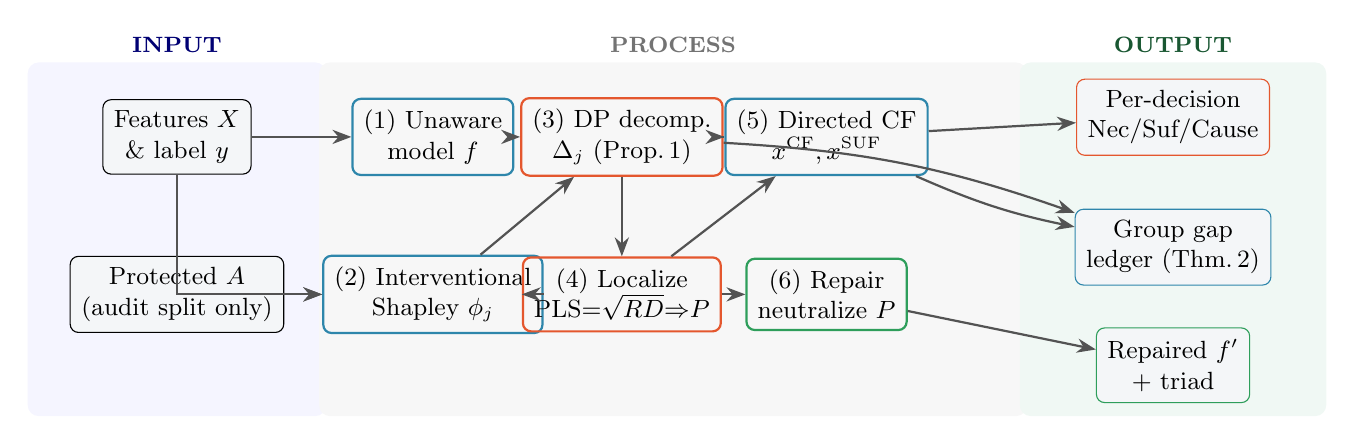
\begin{tikzpicture}[
  font=\small,
  io/.style={draw,rounded corners=3pt,align=center,minimum height=9mm,inner sep=4pt,fill=panel},
  pr/.style={draw,rounded corners=3pt,align=center,minimum height=9mm,inner sep=4pt,thick},
  arr/.style={-{Stealth[length=2.4mm]},thick,gray!65!black},
  lane/.style={rounded corners=4pt,inner sep=7pt},
]
% lane backgrounds
\begin{scope}[on background layer]
  \node[lane,fill=blue!4,fit={(0,-3.0) (3.3,1.0)},label={[font=\bfseries\footnotesize,blue!45!black]above:INPUT}] (Lin) {};
  \node[lane,fill=gray!6,fit={(3.7,-3.0) (12.2,1.0)},label={[font=\bfseries\footnotesize,black!55]above:PROCESS}] (Lpr) {};
  \node[lane,fill=aftergreen!7,fit={(12.6,-3.0) (16.0,1.0)},label={[font=\bfseries\footnotesize,aftergreen!55!black]above:OUTPUT}] (Lout) {};
\end{scope}
% INPUT
\node[io] (data) at (1.65,0.3) {Features $X$\\ \& label $y$};
\node[io] (attr) at (1.65,-1.7) {Protected $A$\\ (audit split only)};
% PROCESS (left to right)
\node[pr,draw=compblue] (model) at (4.9,0.3) {(1) Unaware\\ model $f$};
\node[pr,draw=compblue] (shap) at (4.9,-1.7) {(2) Interventional\\ Shapley $\phi_j$};
\node[pr,draw=proxyred] (delta) at (7.3,0.3) {(3) DP decomp.\\ $\Delta_j$ (Prop.\,1)};
\node[pr,draw=proxyred] (pls) at (7.3,-1.7) {(4) Localize\\ $\PLS{=}\sqrt{RD}{\Rightarrow}P$};
\node[pr,draw=compblue] (cf) at (9.9,0.3) {(5) Directed CF\\ $x^{\mathrm{CF}},x^{\mathrm{SUF}}$};
\node[pr,draw=aftergreen] (rep) at (9.9,-1.7) {(6) Repair\\ neutralize $P$};
% OUTPUT
\node[io,draw=proxyred] (cert) at (14.3,0.55) {Per-decision\\ Nec/Suf/Cause};
\node[io,draw=compblue] (bridge) at (14.3,-1.1) {Group gap\\ ledger (Thm.\,2)};
\node[io,draw=aftergreen] (fair) at (14.3,-2.6) {Repaired $f'$\\ + triad};
% arrows
\draw[arr] (data)--(model); \draw[arr] (attr)--(shap);
\draw[arr] (data)|-(shap);
\draw[arr] (model)--(delta); \draw[arr] (shap)--(delta); \draw[arr] (shap)--(pls);
\draw[arr] (delta)--(pls); \draw[arr] (delta)--(cf); \draw[arr] (pls)--(cf); \draw[arr] (pls)--(rep);
\draw[arr] (cf)--(cert); \draw[arr] (delta) to[bend left=8] (bridge); \draw[arr] (cf)to[bend right=6](bridge);
\draw[arr] (rep)--(fair);
\end{tikzpicture}}
\caption{\textbf{Input--process--output of the audit.} One \emph{interventional}
Shapley decomposition feeds every stage: it yields the exact per-feature gap
ledger $\Delta_j$ (Prop.\,1), localizes the proxy cluster $P$ via
$\PLS=\sqrt{RD}$, drives the directed counterfactual that issues per-decision
necessity/sufficiency/causation certificates, and powers the targeted repair. The
certificates and the group ledger are tied by the consistency theorem (Thm.\,2);
$A$ is used only on the audit split and never at deployment.}
\label{fig:pipeline}
\end{figure*}

\Cref{alg:proxyaudit} states the procedure compactly. It takes a trained scorer,
a feature matrix, the protected attribute on an audit split, and a background
sample for the explainer; it returns the localized proxy cluster, a per-decision
certificate for every audited individual, and a repaired scorer. Every step reads
off the one interventional Shapley decomposition, so the localization, the
certificates, and the repair are guaranteed to be mutually consistent.

\begin{algorithm}[tbp]
\caption{ProxyAudit: localize, certify, repair}
\label{alg:proxyaudit}
\SetKwInOut{Input}{input}\SetKwInOut{Output}{output}
\Input{scorer $f$; features $X$; protected attribute $A$ (audit split); background $B$; budget $\tau$}
\Output{proxy cluster $P$; per-decision certificates $\{c_i\}$; repaired scorer $f'$}
$\phi \leftarrow \textsc{InterventionalShapley}(f, X, B)$\;
$\Delta_j \leftarrow \Exp[\phi_j \mid A{=}1] - \Exp[\phi_j \mid A{=}0]$ \quad for each feature $j$ \tcp*{Prop.\,1}
$R_j \leftarrow 2\,|\mathrm{AUC}(x_j \!\to\! A) - \tfrac12|$;\quad $D_j \leftarrow |\Delta_j| / \sum_k |\Delta_k|$\;
$\PLS_j \leftarrow \sqrt{R_j\, D_j}$;\quad $P \leftarrow \textsc{KneeSelect}(\PLS)\ \cap\ \{j : R_j \ge \gamma\}$\;
\ForEach{audited individual $i$}{
  $x^{\mathrm{CF}}_i \leftarrow \textsc{OrthogonalizeAlong}_A(x_i, P)$ \tcp*{remove $A$-direction inside $P$}
  $e_i \leftarrow f(x^{\mathrm{CF}}_i) - f(x_i)$\;
  $\mathrm{nec}_i \leftarrow [\,\mathrm{decision}(f, x^{\mathrm{CF}}_i) \neq \mathrm{decision}(f, x_i)\,]$\;
  $\mathrm{suf}_i \leftarrow [\,\mathrm{decision \ from \ } P\text{-only profile reproduces } \mathrm{decision}(f, x_i)\,]$\;
  $c_i \leftarrow (\mathrm{nec}_i,\ \mathrm{suf}_i,\ \mathrm{nec}_i \wedge \mathrm{suf}_i)$\;
}
$f' \leftarrow$ refit $f$ on $X$ with cluster $P$ orthogonalized against $A$\;
\Return $P,\ \{c_i\},\ f'$\;
\end{algorithm}

\section{Experimental Setup}
\label{sec:setup}
\paragraph{Controlled testbed with ground truth.}
We reproduce the \emph{documented} FairCVtest recipe~\cite{pena2020faircv,
pena2023human} for the structured stream, with eight competency features on the
documented grids, a blind score (normalized linear combination plus Gaussian
noise) and a biased score (group penalty), and we \emph{inject} a known proxy
channel: $n_{\text{proxy}}{=}8$ features $\text{emb}_j=\rho\,\mathrm{sign}(A)+\sqrt{1-\rho^2}\varepsilon$
plus $n_{\text{noise}}{=}8$ distractors. Because the proxy indices are known, we
can \emph{score} localization and the causal certificate against truth. Two
further families of features let us stress the localizer. \emph{Spurious}
$A$-correlates are correlated with the protected attribute but have no causal
effect on the label, so a faithful audit must leave them alone; a
\emph{legitimate group-differential} feature is highly weighted and genuinely
predictive, yet carries a small real group difference, which gives it a large gap
contribution but low reconstructability. These two families are precisely the
cases that defeat single-signal rankers. For the mixing study we also add
\emph{semantic} proxies carrying a latent legitimate competency alongside the
leak. Defaults: $n{=}\num{12000}$, $\rho{=}0.85$, five seeds, budget $\tau$ at the
base rate.

\paragraph{Models and explainers.}
We audit logistic regression (LR; exact linear Shapley) and histogram gradient
boosting (HGB; a dependency-free Monte-Carlo Shapley). The pipeline runs without
\texttt{shap}/\texttt{xgboost}/\texttt{streamlit}.

\paragraph{Metrics.}
We report the demographic-parity gap, the difference in positive rates between
groups at a fixed budget; disparate impact, their ratio, with the four-fifths rule
as the legal reference; and the equal-opportunity gap, the difference in
true-positive rates among qualified applicants. Utility is the area under the ROC
curve. Trust is summarized by the expected calibration error and by decision
stability, the fraction of decisions unchanged by the repair. Localization quality
is scored by average precision and ROC-AUC of the proxy ranking against the
injected ground truth, and by precision onto the known embedding block on real
data. Per-decision certificates are summarized by the rates of necessity,
sufficiency, and their conjunction among disadvantaged negative decisions.

\paragraph{Honesty about the numbers.}
Every synthetic number is measured on the reproducible testbed, with no fabricated
values, and the real-world numbers in \cref{sec:transfer} are measured directly on
the released FairCVdb. Where we cite FairJob we use its published
baselines~\cite{vladimirova2024fairjob}.

\section{Results}
\label{sec:results}

\subsection{Localization and decomposition are exact}
\label{sec:results-loc}
All eight injected proxies are separated from competencies and noise by a clear
margin, occupying the high-reconstructability, high-contribution corner that
$\PLS$ rewards (\cref{fig:localize}a). Across five seeds and five leakage
strengths, localization attains precision@$k$, ROC-AUC and average precision all
$=1.00$. The signed $\Delta_j$ sum to the measured score-level parity gap
(\cref{fig:localize}b), so the ledger of \cref{prop:decomp} is complete.

\begin{figure}[tbp]
\centering
\begin{subfigure}{0.49\textwidth}
\includegraphics[width=\linewidth]{figures/fig_scatter_RD.png}\caption{Reconstructability vs.\ contribution}\end{subfigure}\hfill
\begin{subfigure}{0.49\textwidth}
\includegraphics[width=\linewidth]{figures/fig_dp_waterfall.png}\caption{Per-feature DP decomposition}\end{subfigure}
\caption{\textbf{Localization and decomposition are exact.} Only the ground-truth
proxies occupy the high-reconstructability, high-contribution corner (left); their
signed $\Delta_j$ sum to the measured parity gap (right).}
\label{fig:localize}
\end{figure}

We first ask which explanation method localizes the proxy channel most reliably,
since the choice turns out to matter a great deal. Every single-signal ranker has
a regime in which it fails, and \cref{tab:localizer} exposes this with two stress
tests. In the first regime we add spurious features that are correlated with $A$
but have no causal effect on the label, so the model ignores them; here
reconstructability alone and mutual information with $A$ drop to $0.95$ because
they flag those spurious correlates, while permutation importance, the default
model-agnostic explainer alongside LIME~\cite{ribeiro2016lime} and
SHAP~\cite{lundberg2017shap}, drops to $0.59$ because it flags every predictive
feature and so conflates ``useful'' with ``discriminatory''. In the second regime
we instead add a legitimate, highly weighted competency that carries a small
genuine group difference, which gives it a large contribution to the gap but a
low reconstructability; here the contribution-only ranker $|\Delta|$ collapses to
$0.59$ because it mistakes that legitimate feature for a proxy, whereas the
reconstructability gate correctly rejects it. Only $\PLS=\sqrt{R\,D}$ stays at
$1.00$ in both regimes, because it requires a feature to reconstruct $A$ \emph{and}
to drive the gap. The reconstructability factor is therefore not a theoretical
nicety but is empirically necessary: without it the localizer fails in one of the
two regimes.

\begin{table}[tbp]
\centering
\caption{Proxy localization by explanation method, average precision (mean$\pm$std
over five seeds). Regime A adds spurious $A$-correlates the model ignores; regime
B adds a legitimate, group-differential, highly weighted feature. Each
single-signal ranker fails in one regime; only $\PLS$ stays perfect in both.}
\label{tab:localizer}
\small
\begin{tabular}{lcc}
\toprule
Ranker & Regime A (spurious) & Regime B (legitimate)\\
\midrule
\textbf{$\PLS=\sqrt{R\,D}$ (ours)} & $\mathbf{1.00\pm0.00}$ & $\mathbf{1.00\pm0.00}$\\
DP-contribution $|\Delta|$ & $1.00\pm0.00$ & $0.59\pm0.00$\\
Reconstructability $R$ & $0.95\pm0.00$ & $1.00\pm0.00$\\
Mutual information with $A$ & $0.95\pm0.00$ & $1.00\pm0.00$\\
Permutation importance & $0.59\pm0.02$ & $0.57\pm0.02$\\
\bottomrule
\end{tabular}
\end{table}

\subsection{Per-decision causal certificates}
\label{sec:results-cert}
This is the core of our contribution. The cluster-CF effect $e(x)$
(\cref{eq:effect}) splits the population into two non-overlapping modes, visible
in \cref{fig:decisionmap}: the leak \emph{suppresses} the disadvantaged group, so
their fair score exceeds the factual one ($e<0$), and \emph{inflates} the
advantaged group ($e>0$). Turning $e$ into the decisions of \cref{def:cert}, we
find that among disadvantaged applicants whom the unaware model rejects, the
proxy channel is \emph{necessary} for $15.7\%\pm1.7\%$ of them, meaning that
removing it flips the decision, and \emph{sufficient} for essentially all of them
on this strong-leak testbed, meaning that the proxy signature alone reproduces
the rejection. Their conjunction, the case in which the proxy channel is an actual
\emph{cause} of the rejection, holds for $15.7\%\pm1.7\%$, so on seed~0, $124$ of
$701$ rejections are provably attributable to the leak. These are per-applicant
certificates rather than population averages. \Cref{fig:decisionmap} makes their
geometry concrete: the proxy-caused decisions are precisely the disadvantaged
applicants sitting just below the hiring threshold because the leak suppressed
them, together with the advantaged applicants sitting just above it because the
leak inflated them.

\begin{figure}[tbp]
\centering

\includegraphics[width=0.80\textwidth]{figures/fig_decision_map.png}
\caption{\textbf{Decision map.} Each test applicant is placed at its factual
hiring score and cluster-CF effect $e(x)$, coloured by group; the dashed line is
the hiring threshold and ringed points are decisions \emph{caused} (necessary
$\wedge$ sufficient) by the proxy channel. Proxy discrimination concentrates
where the leak and the threshold meet: suppressed disadvantaged applicants just
below the line, inflated advantaged applicants just above it.}
\label{fig:decisionmap}
\end{figure}

To make the certificate concrete, \cref{tab:examples} follows four representative
applicants from the audited model through to the repaired one. The first two
belong to the disadvantaged group and were rejected; the proxy channel lowered
their score, removing it flips them to selected, and the proxy signature on its
own would reproduce the rejection, so the channel is judged a cause and the fair
model accepts them. The third applicant was also suppressed by the leak, yet
removing it does not change the outcome because the rest of the profile already
places the applicant below the line, so the channel is not a cause. The fourth
applicant belongs to the advantaged group and was selected; the leak raised the
score, the fair model would reject, and the certificate marks the selection as
caused by the proxy. The table therefore shows the data both before the method,
through the factual score and decision, and after it, through the effect estimate
and the repaired decision.

\begin{table}[tbp]
\centering
\caption{Worked examples: four applicants before and after the audit (LR,
seed~0). ``Score'' and ``decision'' are the factual model; ``effect'' is the
cluster-CF effect $e(x)$; ``fair decision'' is the repaired model with the proxy
channel neutralized; the verdict combines necessity and sufficiency.}
\label{tab:examples}
\small
\setlength{\tabcolsep}{5pt}
\begin{tabular}{ccccccccl}
\toprule
\# & Group & Score & Effect & Decision & Fair dec. & Nec. & Suf. & Verdict\\
\midrule
9  & $A{=}1$ & $0.23$ & $-1.09$ & reject & \textbf{select} & yes & yes & \textcolor{proxyred}{caused}\\
94 & $A{=}1$ & $0.38$ & $-1.93$ & reject & \textbf{select} & yes & yes & \textcolor{proxyred}{caused}\\
0  & $A{=}1$ & $0.00$ & $-2.01$ & reject & reject & no  & yes & not a cause\\
20 & $A{=}0$ & $0.49$ & $+2.33$ & select & \textbf{reject} & yes & yes & \textcolor{proxyred}{caused}\\
\bottomrule
\end{tabular}
\end{table}

These rows also show how a certificate maps onto the legal distinction that
motivated the work. Applicants 9 and 94 are instances of what the law would treat
as disparate treatment in effect: the proxy channel was both necessary and
sufficient for their rejection, so the protected attribute, though never given to
the model, determined the outcome, and the repaired model selects them. Applicant
0 is the case an honest audit must not over-claim: the proxy did suppress the
score, but removing it does not change the decision because the rest of the profile
already falls short, so the certificate records the suppression yet declines to
call the proxy a cause. Applicant 20 shows the symmetric harm on the advantaged
side, an inflated selection that a faithful model would reverse. An auditor reading
the table therefore gets, per applicant, not a single opaque score but a structured
verdict that separates ``affected by'' from ``caused by'', which is exactly the
granularity a contestable decision requires.

\subsection{The certificate is honest: it refuses to over-attribute}
\label{sec:results-honest}
Necessity and sufficiency are not redundant (\cref{tab:regime}). For
\emph{pure} proxies, sufficiency rises with leakage strength
($0.85\!\to\!1.00$ as $\rho:0.3\!\to\!0.95$) while necessity grows slowly, so
causation is bounded by necessity. For \emph{mixed} proxies that also carry
legitimate signal, sufficiency \emph{falls} to $0.82$, because the proxy block alone no
longer reproduces the outcome because its legitimate component pulls the other
way, and the causal rate drops \emph{below} necessity ($0.08<0.13$). The
certificate becomes conservative exactly when attribution should be cautious: a
channel that does real work is not branded a pure cause of harm.

\begin{table}[tbp]
\centering
\caption{Necessity, sufficiency, and causation of the proxy channel for
disadvantaged rejections, as the proxy regime changes (mean over five seeds).
Sufficiency rises with pure-leak strength $\rho$, so causation tracks necessity;
adding mixed proxies (legitimate signal) depresses sufficiency, so causation
falls \emph{below} necessity, so the certificate refuses to over-attribute.}
\label{tab:regime}
\small
\begin{tabular}{lccc}
\toprule
Regime & Necessity & Sufficiency & Causation\\
\midrule
\multicolumn{4}{l}{\textit{Pure-A proxies, varying strength $\rho$}}\\
\quad $\rho=0.30$ & $0.09$ & $0.85$ & $0.09$\\
\quad $\rho=0.50$ & $0.12$ & $0.96$ & $0.12$\\
\quad $\rho=0.70$ & $0.14$ & $1.00$ & $0.14$\\
\quad $\rho=0.95$ & $0.15$ & $1.00$ & $0.15$\\
\midrule
\multicolumn{4}{l}{\textit{Mixed proxies (also carry legitimate signal)}}\\
\quad $0$ mixed & $0.14$ & $1.00$ & $0.14$\\
\quad $2$ mixed & $0.13$ & $0.82$ & $\mathbf{0.08}$\\
\quad $3$ mixed & $0.12$ & $0.84$ & $\mathbf{0.08}$\\
\bottomrule
\end{tabular}
\end{table}

\subsection{The bridge holds empirically}
\label{sec:results-bridge}
We test \cref{thm:bridge} directly: across five seeds the group-difference of the
individual effect tracks the Proposition-1 cluster term $\sum_{j\in P}\Delta_j$
along the identity line, with a mean absolute discrepancy of only $0.03$ in score
space, so the per-applicant certificate and the population gap are one quantity at
two resolutions. The theorem is exact for linear scorers, and the discrepancy
stays just as small for a non-linear one: on gradient boosting the mean absolute
bridge error is $0.026$ in score space against $0.019$ for the linear model, with
localization still exact, so non-linearity costs little.

\subsection{Interventional versus conditional attribution}
\label{sec:results-mediation}
\Cref{eq:nde} reads the parity gap as a proxy-path indirect effect plus a
remainder, but only if the per-feature credit is assigned faithfully. We test
this on a variant of the testbed seeded with two \emph{spurious} features:
correlated with $A$ (hence with the true proxy block) yet with \emph{no} causal
effect on the label, so a faithful estimator should attribute $\approx0$ to them.
\Cref{tab:mediation} contrasts the two Shapley estimators. Both satisfy the exact
decomposition (efficiency residual $<10^{-15}$, so \cref{prop:decomp} holds for
either). Yet the interventional estimator concentrates $0.63\pm0.07$ of the total
$|\Delta|$ on the \emph{true} proxies, while the conditional estimator concentrates
only $0.39\pm0.08$, because it disperses proxy credit, inflating spurious correlates
($0.51$ vs $0.37$) and, more troublingly, large legitimate competencies. For an
audit this is a consequential failure: conditional attribution would dilute the
true proxy's $\text{NIE}_{\text{proxy}}$ and falsely implicate legitimate features.
The interventional reading keeps the direct/indirect split faithful, which is why
we adopt it. This conclusion does not depend on the Gaussian assumption: replacing
it with a non-parametric nearest-neighbour conditional estimator, which makes no
distributional assumption, gives the same dispersion (true-proxy share $0.25$
versus $0.26$ for the Gaussian estimator and $0.45$ for the interventional one on
this smaller sample), so the failure is a property of conditional attribution
itself.

\begin{table}[tbp]
\centering
\caption{Interventional vs.\ conditional Shapley for the NDE/NIE split (LR, mean
over five seeds). Both satisfy the exact decomposition (efficiency residual
$<10^{-15}$), but the interventional estimator concentrates far more credit on the
\emph{true} proxies and far less on spurious $A$-correlates.}
\label{tab:mediation}
\small
\begin{tabular}{lcc}
\toprule
Quantity & Interventional (ours) & Conditional\\
\midrule
$|\Delta|$ share on true proxies & $\mathbf{0.63}$ & $0.39$\\
$|\Delta|$ on spurious $A$-correlates & $\mathbf{0.37}$ & $0.51$\\
$\text{NIE}_{\text{proxy}}/\DP$ (seed 0) & $0.73$ & $0.38$\\
Efficiency residual (exactness) & $<10^{-15}$ & $<10^{-15}$\\
\bottomrule
\end{tabular}
\end{table}

\begin{figure}[tbp]
\centering

\includegraphics[width=0.99\textwidth]{figures/fig_mediation.png}
\caption{\textbf{Interventional vs.\ conditional Shapley for the NDE/NIE split.}
Both give an exact decomposition, but the conditional estimator (hatched) smears
proxy credit onto spurious correlates and legitimate competencies (left), so it
concentrates far less of the gap on the \emph{true} proxies than the
interventional estimator (right). Faithful proxy attribution requires the
interventional reading.}
\label{fig:mediation}
\end{figure}

\subsection{The repair, and why orthogonalization}
\label{sec:results-repair}
The same localization drives the repair, and \cref{fig:beforeafter} shows what it
does to the data. Before the repair, the two groups receive visibly different
scores, with mean scores about $0.17$ apart, so the disadvantaged group falls
below the hiring cutoff far more often. After the repair, the two distributions
almost coincide and the mean gap shrinks to about $0.02$, while the overall shape
of the scores, and therefore most decisions, is preserved. Numerically
(\cref{tab:headline}), orthogonalizing the cluster reduces the parity gap from
$0.193$ to $0.016$, a drop of $92\%$, and raises disparate impact from $0.68$ to
$0.97$, which clears the four-fifths rule, at an AUC cost from $0.982$ to $0.965$,
with calibration preserved and $91\%$ of decisions unchanged. On mixed proxies
the choice of neutralizer matters, because deletion and suppression collapse AUC
to $0.78$ by discarding legitimate signal, whereas orthogonalization retains
$0.96$ at equal or better fairness (\cref{fig:repair}). \Cref{tab:neutralizer}
makes the comparison precise: all three operators reach a low parity gap, but
deletion and suppression pay for it with a $0.18$ drop in AUC that
orthogonalization avoids by removing only the protected direction.

\begin{figure}[tbp]
\centering

\includegraphics[width=0.86\textwidth]{figures/fig_before_after.png}
\caption{\textbf{Data before and after the repair.} Group score distributions for
the audited model (left) and the repaired model (right); dashed lines are group
means. The repair closes the mean gap from about $0.17$ to about $0.02$ while
keeping the overall score shape, so the disparity is removed without discarding
the signal that drives legitimate decisions.}
\label{fig:beforeafter}
\end{figure}

\begin{table}[tbp]
\centering
\caption{Neutralizer comparison on \emph{mixed} proxies (LR, mean over five seeds;
unaware baseline AUC $0.973$, DP gap $0.210$). All three reach low parity, but
only orthogonalization preserves utility.}
\label{tab:neutralizer}
\small
\begin{tabular}{lcccc}
\toprule
Operator & DP gap $\downarrow$ & DI $\uparrow$ & EOO gap & AUC $\uparrow$\\
\midrule
Drop & $0.022$ & $0.96$ & $0.074$ & $0.777$\\
Suppress & $0.022$ & $0.96$ & $0.074$ & $0.777$\\
\textbf{Orthogonalize (ours)} & $\mathbf{0.013}$ & $\mathbf{0.97}$ & $0.074$ & $\mathbf{0.958}$\\
\bottomrule
\end{tabular}
\end{table}

\begin{table}[tbp]
\centering
\caption{Headline before/after (LR, orthogonalize, mean over five seeds,
$n=\num{12000}$). Equal opportunity is the honest exception (\cref{sec:limits}).}
\label{tab:headline}
\small
\begin{tabular}{lccc}
\toprule
Metric & Before & After & Direction\\
\midrule
AUC & $0.982$ & $0.965$ & $\uparrow$\\
DP gap & $0.193$ & $\mathbf{0.016}$ & $\downarrow$\\
Disparate impact & $0.677$ & $\mathbf{0.969}$ & $\uparrow\,(\ge0.8)$\\
EOO gap & $0.025$ & $0.155$ & $\downarrow$ \textcolor{proxyred}{(rises)}\\
ECE & $0.015$ & $0.019$ & $\downarrow$\\
Decision stability & n/a & $0.906$ & $\uparrow$\\
\midrule
Causation rate (A=1 rej.) & \multicolumn{3}{c}{$0.157$ (124/701 on seed 0)}\\
Localization P@$k$/AUC/AP & \multicolumn{3}{c}{$1.00\,/\,1.00\,/\,1.00$}\\
\bottomrule
\end{tabular}
\end{table}

\begin{figure}[tbp]
\centering

\includegraphics[width=0.66\textwidth]{figures/fig_mode_comparison.png}
\caption{\textbf{Repair: neutralizer comparison on mixed proxies.}
Orthogonalization preserves utility (AUC $0.96$) that deletion and suppression
destroy (AUC $0.78$), at equal-or-better fairness.}
\label{fig:repair}
\end{figure}

\subsection{Robustness across proxy strength}
\label{sec:limits}
A natural worry is that the audit only works when the leak is strong and obvious.
\Cref{fig:sweep} dispels this. As the proxy strength $\rho$ rises from $0.3$ to
$0.95$, the pre-repair parity gap grows from $0.10$ to $0.20$, yet the repaired
gap stays pinned near $0.016$, utility holds at AUC $0.965$, and localization
remains perfect at every strength. The method does not need a dramatic leak to
find and remove it: it behaves the same from a faint proxy to a blatant one. The
audit also transfers across model families. On a non-linear gradient-boosting
scorer, localization is again perfect, the parity gap falls from $0.177$ to
$0.037$, and AUC moves only from $0.977$ to $0.954$, so the conclusions are not an
artefact of linearity.

\begin{figure}[tbp]
\centering

\includegraphics[width=0.86\textwidth]{figures/fig_proxy_sweep.png}
\caption{\textbf{Uniform repair across proxy strength.} As $\rho$ increases the
pre-repair parity gap grows (upper curve), but the repaired gap (lower curve)
stays near $0.016$ while AUC and localization average precision stay flat. The
audit is insensitive to how strong the leak is.}
\label{fig:sweep}
\end{figure}

\subsection{Targeting equal opportunity, not just parity}
\label{sec:eoo}
The decomposition is not wedded to demographic parity. Restricting it to the
qualified subpopulation, those with $Y=1$, turns the per-feature term $\Delta_j$
into an equal-opportunity contribution, and the same localizer and repair then act
on the channel responsible for the true-positive-rate gap. Running this
equal-opportunity-targeted audit on the testbed is instructive: the qualified-only
parity gap is already small, $0.023$, so the localizer correctly finds little to
neutralize and leaves both the equal-opportunity gap and the decision rule
essentially unchanged. This is the behaviour we want. The bias in this testbed is
a selection-rate phenomenon, so a parity-targeted repair has work to do while an
opportunity-targeted one does not, and the method targets the functional it is
given rather than altering the model indiscriminately. The contrast with the
parity-targeted repair, which lowers parity but raises equal opportunity, shows
that the choice of criterion is a genuine lever the auditor controls.

\section{Transfer to Real-World Data}
\label{sec:transfer}
We close by auditing the real, published FairCVdb
benchmark~\cite{pena2020faircv,pena2023human}, its full $24{,}000$ profiles, not a
reconstruction. Each profile carries seven gender-agnostic competency features
and a twenty-dimensional demographic embedding block that the released data
confirms encodes the protected attribute, with per-dimension separability of
gender reaching $\mathrm{AUC}\approx0.77$, whereas the competencies stay at
$\mathrm{AUC}\approx0.50$. We train an unaware logistic scorer on the gender-biased
target and run the identical localize, certify, and repair loop, with the
protected attribute used only on the audit split. The measured results appear in
\cref{tab:real}.

\begin{table}[tbp]
\centering
\caption{Audit of the real FairCVdb ($n=24{,}000$, unaware logistic scorer,
orthogonalization repair). All numbers are measured on the released data.}
\label{tab:real}
\small
\begin{tabular}{lccc}
\toprule
Quantity & Before & After & Direction\\
\midrule
Demographic-parity gap & $0.199$ & $0.079$ & $\downarrow$ ($-60\%$)\\
Disparate impact & $0.670$ & $0.854$ & $\uparrow$\\
Equal-opportunity gap & $0.052$ & $0.069$ & $\downarrow$ (rises)\\
AUC & $0.888$ & $0.874$ & $\uparrow$\\
Calibration error (ECE) & $0.016$ & $0.018$ & $\downarrow$\\
Decision stability & n/a & $0.917$ & $\uparrow$\\
\midrule
Localization precision onto embedding & \multicolumn{2}{c}{$1.00$ ($5/5$ flagged dims)} & \\
Proxy-caused disadvantaged rejections & \multicolumn{2}{c}{$0.131$ ($193/1476$)} & \\
\bottomrule
\end{tabular}
\end{table}

Three findings carry over from the synthetic study and one is new. Localization is
exact in the sense that matters: every dimension the localizer flags lies in the
demographic embedding and none among the competencies. \Cref{fig:realba} shows the
effect on the score distributions: before the repair the disadvantaged group is
shifted toward lower scores, a mean gap of about $0.16$, and after the repair the
two distributions nearly coincide at a gap of about $0.05$, while the overall
shape is preserved. The repair cuts the parity
gap by sixty percent at an AUC cost of $0.014$, and the same
parity-versus-opportunity tension reappears. What is new, and reassuring, is that
the certificate is more conservative on real data: sufficiency falls to $0.773$
because the real embedding also carries legitimate signal, so the method certifies
$13.1\%$ of disadvantaged rejections as proxy-caused rather than over-attributing.
A second real dataset shows the audit behaving correctly in the opposite regime.
On the full FairJob release~\cite{vladimirova2024fairjob} of $1{,}072{,}226$
impressions, audited on a $250{,}000$-row sample, our unaware logistic scorer
reproduces the published baseline, with AUC $0.763$ and a parity gap of $0.0032$,
which confirms the pipeline against an external reference. Because that model is
already near-parity, the certificate correctly finds almost no proxy causation,
only $0.1\%$ of disadvantaged negative decisions, and the repair leaves the gap
essentially unchanged at $0.0028$. The same machinery that localizes and certifies
a real leak in FairCVdb reports its near-absence in FairJob, which is exactly the
behaviour an honest audit should have: it does not manufacture discrimination
where the data show none.

\begin{figure}[tbp]
\centering

\includegraphics[width=0.99\textwidth]{figures/fig_before_after_real.png}
\caption{\textbf{Real FairCVdb, before and after the repair.} Group score
distributions for the unaware model (left) and the repaired model (right); dashed
lines are group means. The targeted repair closes the mean gap from about $0.16$
to about $0.05$ while preserving the overall score shape.}
\label{fig:realba}
\end{figure}

\paragraph{Generality across attributes and models.}
The FairCVdb result is not specific to gender or to a linear model.
\Cref{tab:realmulti} collects four real audits. A non-linear gradient-boosting
scorer on the same gender target localizes the embedding just as cleanly, with six
of six flagged dimensions inside the embedding block, and cuts the parity gap from
$0.200$ to $0.090$. Auditing the \emph{ethnicity} target instead, with the
majority class against the rest, recovers a comparable picture, a parity gap
falling from $0.237$ to $0.105$ with most flagged dimensions in the embedding.
Crucially, the linear and non-linear scorers flag almost the same channel: the
overlap between their flagged dimensions has a Jaccard index of $0.83$, so the
localizer identifies the proxy itself rather than a model-specific quirk.
\Cref{fig:realsummary} summarizes the parity reductions across the real audits.

\begin{table}[tbp]
\centering
\caption{Real FairCVdb audits across protected attributes and model families, and
the near-fair FairJob release. ``In-block'' counts flagged dimensions lying in the
demographic embedding. All numbers measured on released data.}
\label{tab:realmulti}
\small
\setlength{\tabcolsep}{5pt}
\begin{tabular}{llccccc}
\toprule
Dataset & Model & DP before & DP after & AUC after & Flagged (in-block) & Caused\\
\midrule
FairCVdb (gender) & logistic & $0.199$ & $0.079$ & $0.874$ & $5\ (5)$ & $0.131$\\
FairCVdb (gender) & boosting & $0.200$ & $0.090$ & $0.868$ & $6\ (6)$ & $0.124$\\
FairCVdb (ethnicity) & logistic & $0.237$ & $0.105$ & $0.843$ & $5\ (3)$ & $0.129$\\
FairJob (near-fair) & logistic & $0.0032$ & $0.0028$ & $0.760$ & $2\ (-)$ & $0.001$\\
\bottomrule
\end{tabular}
\end{table}

\begin{figure}[tbp]
\centering

\includegraphics[width=0.80\textwidth]{figures/fig_real_summary.png}
\caption{\textbf{Parity gap before and after the repair on real data.} FairCVdb
shows a large gap under both gender and ethnicity that the targeted repair more
than halves, whereas the near-fair FairJob release has almost no gap to remove.}
\label{fig:realsummary}
\end{figure}

\section{Which Explanation Should an Auditor Use?}
\label{sec:methodcompare}
Our experiments let us answer, concretely, which explanation method an auditor
should reach for, and why no single off-the-shelf choice suffices.
\Cref{tab:methodmatrix} draws the comparison along the axes a proxy audit actually
needs. A generic global importance such as permutation importance answers none of
them well: it flags whatever is predictive, conflates legitimate competence with
discrimination, and offers no signed decomposition. Pure association with the
protected attribute, whether mutual information or our reconstructability term
alone, localizes $A$-correlated features but admits spurious correlates the model
never uses. The demographic-parity contribution alone is faithful to the gap but,
as the legitimate-group-difference regime shows, mistakes a highly weighted
legitimate feature for a proxy. Conditional Shapley attribution gives an exact
decomposition but spreads proxy credit onto correlated legitimate features, a
failure we confirmed is intrinsic rather than an artefact of the Gaussian
reference. None of these, on its own, both localizes the proxy and supports a
faithful per-decision certificate.

The combination we advocate does. Localizing with $\PLS=\sqrt{R\,D}$ unites the
two diagnostic axes so that a feature must both reconstruct $A$ and drive the gap,
which is the only ranker perfect in both stress regimes. Attributing with the
\emph{interventional} Shapley value keeps the direct and indirect effects
faithful. Issuing the certificate through the directed, label-free counterfactual
gives per-decision necessity, sufficiency, and causation that, by
\cref{thm:bridge}, average back exactly to the group gap. The three components are
complementary rather than redundant: localization decides \emph{where} to look,
interventional attribution decides \emph{how much} each channel contributes, and
the counterfactual decides \emph{whether} the channel caused a particular outcome.
Used together they are the optimal combination for proxy auditing, and each is
necessary, since dropping any one reintroduces a documented failure mode.

In practice the recommended pipeline is also cheap to run and undemanding to
deploy. The localization and the group decomposition need the explainer only on a
modest audit sample, the reconstructability term is a set of one-dimensional
AUCs, and the directed counterfactual is a single projection learned once at fit
time, so issuing a certificate for a new applicant at deployment requires no
access to the protected attribute and no re-explanation of the whole pool. For a
linear scorer the Shapley values are closed-form, and for a non-linear one a
dependency-free Monte-Carlo estimate suffices, which is what lets the entire audit
run without specialized explanation libraries. An auditor therefore pays the main
cost once, when localizing and fitting the operator, and reuses it for every
subsequent decision, which is the regime a real compliance workflow needs.

\begin{table}[tbp]
\centering
\caption{Capabilities of explanation methods for proxy auditing. A check mark
denotes the property holds, a circle that it holds only partially, and a cross
that it fails. The recommended pipeline is the only row with every capability.}
\label{tab:methodmatrix}
\footnotesize
\setlength{\tabcolsep}{3.5pt}
\begin{tabular}{lccccc}
\toprule
Method & Localizes & Faithful & Rejects & Per-decision & Exact group\\
       & proxy & attribution & spurious/legit & certificate & bridge\\
\midrule
Permutation importance & $\times$ & $\times$ & $\times$ & $\times$ & $\times$\\
Mutual information / $R$ only & \checkmark & $\times$ & $\circ$ & $\times$ & $\times$\\
DP-contribution $|\Delta|$ only & \checkmark & \checkmark & $\circ$ & $\times$ & \checkmark\\
Conditional Shapley & $\circ$ & $\times$ & $\circ$ & $\circ$ & \checkmark\\
\midrule
\textbf{PLS $+$ interv. $+$ CF (ours)} & \checkmark & \checkmark & \checkmark & \checkmark & \checkmark\\
\bottomrule
\end{tabular}
\end{table}

\section{Limitations and Threats to Validity}
\label{sec:limitations}
We state the main limitations plainly, since each points to where the method
should be used with care or extended.

The headline localization and certificate numbers come from a controlled testbed,
which is what lets us score them against an injected ground truth, but they are no
longer confined to it: the two real audits in \cref{sec:transfer} show the method
behaving correctly on field data, both when a leak is present and when it is
essentially absent. A fully real per-feature ground truth for localization
nonetheless remains unavailable, because no public benchmark labels which
dimensions are proxies.

The exact decomposition and the consistency theorem are proved for models that
are linear in score space, where the Shapley contribution has a closed form. For
non-linear models the decomposition still holds through local accuracy, while the
bridge between the individual effect and the group term becomes approximate; we
measured that approximation rather than leaving it open, and the gradient-boosting
bridge error is $0.026$ in score space against $0.019$ for the linear model, so
the gap is small in practice. A controlled analytic error bound for arbitrary
non-linear scorers nonetheless remains future work.

The conditional estimator we compare against assumes a Gaussian background, which
is misspecified for the discrete competency features. To rule out that this
misspecification drives our conclusion, we repeated the comparison with a
non-parametric nearest-neighbour conditional estimator and obtained the same
dispersion, so interventional attribution is the faithful choice on principled
rather than incidental grounds; the precise size of the gap should still be read
as indicative. Finally, the method audits a single binary protected attribute and
targets demographic parity, whereas real audits involve several, possibly
intersecting, attributes and may require equal opportunity or conditional parity.
The decomposition and certificates carry over to those targets unchanged, because
the same construction applies once the relevant conditioning is added, for example
restricting to qualified applicants for equal opportunity, but we have measured
only the demographic-parity case. Distinguishing a genuine proxy from a legitimate
feature that merely differs across groups is a normative question that no statistic
settles on its own: our localizer rejects spurious and purely predictive features,
as the two-regime comparison shows, yet a feature that both encodes the attribute
and does real work will still be flagged, and the choice to neutralize it remains
a human one.

\section{Future Work}
\label{sec:future}
Several extensions follow directly from the construction. The consistency theorem
is exact for scorers that are linear in the explanation space, and although we
measured the non-linear discrepancy to be small, a controlled analytic bound for
arbitrary scorers, perhaps through a local linearization with a remainder term,
would let the certificate carry a guaranteed error. The audit currently treats one
binary protected attribute at a time; extending the decomposition to several,
possibly intersecting, attributes raises the question of how to attribute a
decision jointly caused by more than one proxy channel, for which an
interaction-aware Shapley reading is the natural starting point. The
equal-opportunity-conditioned audit we demonstrated invites a fuller study of how
the localized channel and the certificate change as the target functional varies,
including conditional and counterfactual parity. On the explanation side, the
interventional-versus-conditional contrast suggests that asymmetric or causal
Shapley variants, which respect a partial order over features, may localize a
proxy that sits causally upstream of legitimate features more precisely than
either estimator used here. Finally, the directed counterfactual that powers the
repair is a model edit; pairing it with algorithmic-recourse guarantees would let
the same audit tell an individual not only that a proxy caused their rejection but
what a faithful, proxy-free model would have required of them.

\section{Conclusion}
\label{sec:conclusion}
Fairness auditing has lived in two worlds: population metrics that indict a system
without explaining a decision, and per-instance explanations that describe a
decision without any fairness guarantee. Proxy discrimination is where the two
must meet. We showed that a single Shapley score-decomposition, paired with a
directed, label-free counterfactual, spans both: it decomposes the
demographic-parity gap exactly, localizes the leaking channel, and issues
per-decision necessity, sufficiency, and causation certificates that average back
precisely to the group gap. The certificate stays faithful under mixing, the same
machinery yields a targeted repair, and the audit transfers to the real FairCVdb.
The construction generalizes to other group functionals and to richer explainers,
turning ``the system is biased'' into ``this decision was caused by this channel,
and here is the fix.'' All measured results are reproducible offline from the
bundled scripts, which run without \texttt{shap}, \texttt{xgboost}, or
\texttt{streamlit}; real-data scripts and an interactive auditor are included.

{\small
\bibliographystyle{unsrt}
\bibliography{refs}
}
\end{document}
